\begin{table}[t]
\centering\small
\caption{\textbf{Falsifying $\Gamma$ from leniency variation} (SL-Bench, 5
decision makers, 30 configurations). $\Gamma_0^{\mathrm{cond}}$ is the
\emph{within-decision-maker} sensitivity parameter, which is what
\cref{prop:falsify} bounds from below. ``Recovered'' is
$\log\Gamma_{\min}/\log\Gamma_0^{\mathrm{cond}}$ at the robust ($95$th
percentile) variant. The bound was valid in every one of the 30 cells, and never
refuted a true missing-at-random mechanism.}
\label{tab:falsify}
\begin{tabular}{cccccc}
\toprule
target $\Gamma_0$ & reliance on $S$ & $\Gamma_0^{\mathrm{cond}}$ &
$\Gamma_{\min}$ & $\Gamma_{\min}$ (q95) & recovered\\
\midrule
$1.0$ & homogeneous   & $1.000$  & $1.000$ & $1.000$ & --- \\
$1.0$ & heterogeneous & $1.000$  & $1.000$ & $1.000$ & --- \\
$1.5$ & homogeneous   & $1.582$  & $1.423$ & $1.341$ & $0.61$\\
$1.5$ & heterogeneous & $1.862$  & $1.573$ & $1.398$ & $0.51$\\
$2.0$ & homogeneous   & $2.273$  & $1.814$ & $1.594$ & $0.54$\\
$2.0$ & heterogeneous & $2.924$  & $2.181$ & $1.685$ & $0.45$\\
$3.0$ & homogeneous   & $3.831$  & $2.409$ & $1.914$ & $0.45$\\
$3.0$ & heterogeneous & $5.445$  & $3.164$ & $2.047$ & $0.39$\\
$5.0$ & homogeneous   & $7.623$  & $3.171$ & $2.270$ & $0.37$\\
$5.0$ & heterogeneous & $11.195$ & $4.420$ & $2.419$ & $0.34$\\
\bottomrule
\end{tabular}
\end{table}

\paragraph{The test never over-claims, and never cries wolf.}
\Cref{tab:falsify} reports $\Gamma_{\min}$ across 30 configurations varying the
true $\Gamma_0$, the spread of leniency, and whether decision makers rely on
their private information to the same degree. Two properties hold without
exception. First, \emph{validity}: $\Gamma_{\min}\le\Gamma_0^{\mathrm{cond}}$ in
every cell, as \cref{prop:falsify} requires. Second, \emph{no false alarms}: when
the mechanism really is missing-at-random the test returns exactly $1.000$ and
refutes nothing, so an analyst who runs it on genuinely unconfounded data is not
pushed into a needless sensitivity analysis.

\paragraph{How much it recovers.} \Cref{fig:falsify} plots every configuration
against the truth; on the log scale the test recovers $34$--$61\%$
of the truth, and --- as theory predicts --- less when decision makers differ in
\emph{how much} they use their private information rather than only in how
lenient they are: heterogeneity in reliance is exactly what makes different
decision makers' identified sets overlap for smaller $\Gamma$. So
$\Gamma_{\min}$ should be read as what it is: a floor the data will not let you
go below, not an estimate of $\Gamma_0$. At $\Gamma_0=3$ it already refutes
$\dcsm(\Gamma)$ for every $\Gamma<1.9$, which rules out missing-at-random ---
and with it IPW and AIPW --- decisively.

\begin{figure}[t]
\centering
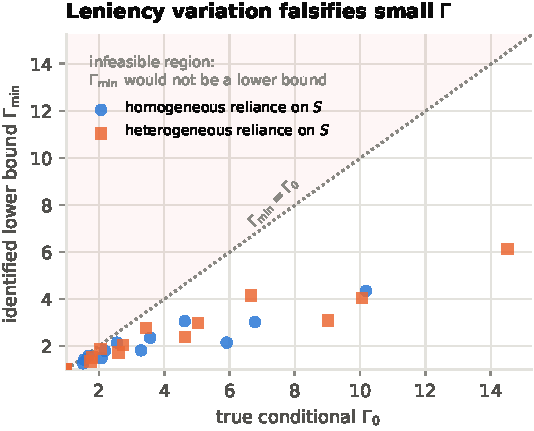
\includegraphics[width=0.58\linewidth]{figures/fig6_falsification}
\caption{\textbf{Every point lies below the diagonal:} the identified lower bound
never exceeds the true conditional $\Gamma_0$. Heterogeneous reliance on private
information across decision makers loosens the bound, as \cref{prop:falsify}'s
intersection argument predicts.}
\label{fig:falsify}
\end{figure}

\paragraph{Break-even analysis: what survives.}
The deliverable a practitioner wants is not a single interval but the $\Gamma$ at
which a conclusion flips. On Lending Club the incumbent model's AUROC lower bound
stays above $0.55$ up to $\Gamma=1.72$ and above chance up to $\Gamma=2.82$ ---
so the claim ``this model ranks better than chance'' survives past the true
$\Gamma_0=2.0$, while the stronger claim ``AUROC is at least $0.60$'' does not
survive even $\Gamma=1.05$. On MIMIC-sim, where the model is far more
discriminative, the above-chance claim survives to $\Gamma=14.9$. Separately, the
DCL model's certified worst-case risk beats the incumbent's at \emph{every}
$\Gamma$ we tested, up to $\Gamma=40$: the ordering of models under the
certificate is robust even where the absolute numbers are not.

\paragraph{When $\Gamma$ is set too small.} \Cref{tab:misspec} shows the failure
mode is graceful. Coverage is $100\%$ for every $\Gamma$ at least half the truth
and falls only to $69\%$ at $\Gamma\le\Gamma_0/2$, while the interval widens
monotonically and slowly --- from $0.04$ to $0.40$ over a $200$-fold range of
$\Gamma$. The price of a conservative $\Gamma$ is a wider interval, not a wrong
one; the price of an aggressive one is a graded loss of coverage, not a cliff.

\begin{table}[t]
\centering\small
\caption{\textbf{Coverage and width when the assumed $\Gamma$ is wrong}
(SL-Bench, 3 seeds, $\Gamma$ swept over a $200$-fold range).}
\label{tab:misspec}
\begin{tabular}{lcccccc}
\toprule
$\Gamma/\Gamma_0$ & $\le 0.5$ & $(0.5, 0.8]$ & $(0.8,1.0]$ & $(1.0,1.5]$ & $(1.5,3]$ & $>3$\\
\midrule
coverage & $0.69$ & $1.00$ & $1.00$ & $1.00$ & $1.00$ & $1.00$\\
mean width & $0.04$ & $0.14$ & $0.21$ & $0.26$ & $0.35$ & $0.40$\\
\bottomrule
\end{tabular}
\end{table}
